\chapter{Dérivation}
\thispagestyle{fancy}

\section{Limite en zéro d'une fonction}

\begin{bexemples}
    \begin{enumEx}
        \item Soit la fonction $f$ définie sur $\left]-\infty ; 0\right[\cup\left] 0 ;+\infty\right[ $ par $f(x)=\dfrac{(x+1)^{2}-1}{x}$. \\
        L'image de 0 par la fonction $f$ n'existe pas. On s'intéresse cependant aux valeurs de $f(x)$ lorsque $x$ se rapproche de $0$.
        \begin{center}
            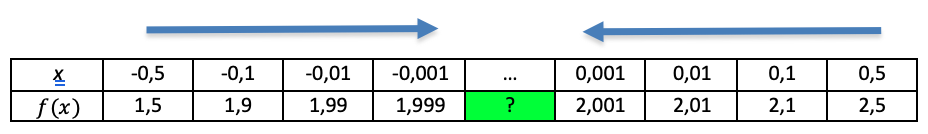
\includegraphics[scale=1]{01-05-Img01}
        \end{center}
        On constate que $f(x)$ se rapproche de 2 lorsque $x$ se rapproche de 0 . On dit que la limite de $f$ lorsque $x$ tend vers 0 est égale à 2 et on note : $\lim \limits_{x \rightarrow 0} f(x)=2$.
        \item Soit la fonction $g$ définie sur $]-\infty ; 0[\cup] 0 ;+\infty[$ par $g(x)=\dfrac{1}{x^{2}}$.\\
        A l'aide de la calculatrice, on constate que $g(x)$ devient de plus en plus grand lorsque $x$ se rapproche de 0
        On dit que la limite de $g$ lorsque $x$ tend vers 0 est égale à $+\infty$ et on note :
        $\lim \limits_{x \rightarrow 0} g(x)=+\infty$
    \end{enumEx}
\end{bexemples}

\begin{bdefi}
    \phantom{$\dfrac{1}{3}$}\pointille[\textwidth-1cm]\\
    \phantom{$\dfrac{1}{3}$}\pointille[\textwidth-1cm]\\
    \phantom{$\dfrac{1}{3}$}\pointille[\textwidth-1cm]\\
    \phantom{$\dfrac{1}{3}$}\pointille[\textwidth-1cm]
\end{bdefi}

\section{Nombre dérivé}

\subsection{Rappel : Pente d'une droite}

Soit une fonction $f$ définie sur un intervalle I. Soit deux réels $a$ et $b$ appartenant à I tels que $a<b$. Soit $\mathrm{A}$ et $\mathrm{B}$ deux points de la courbe représentative de $f$ d'abscisses respectives $a$ et $b$. La pente (ou le coefficient directeur) de la droite (AB) est égal à : $\dfrac{f(b)-f(a)}{b-a}$.

%\begin{center}
%    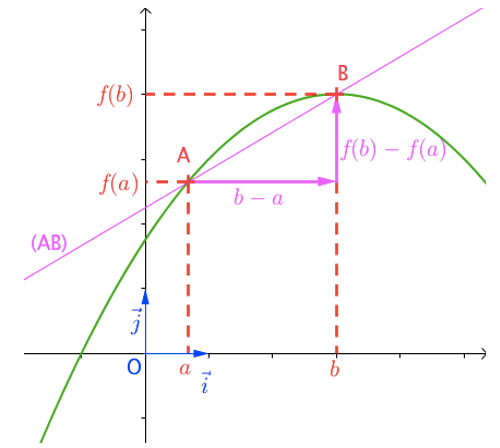
\includegraphics[scale=0.8]{01-05-Img02}
%\end{center}

\subsection{Fonction dérivable}

\begin{multicols}{2}

Soit une fonction $f$ définie sur un intervalle $I .$ Soit un réel $a$ appartenant à I.\\
\ \\
Soit A et M deux points de la courbe représentative de $f$ d'abscisses respectives $a$ et $a+h,$ avec $h \neq 0$
La pente de la droite (AM) est égale à :
$\dfrac{f(a+h)-f(a)}{a+h-a}=\dfrac{f(a+h)-f(a)}{h}$.\\

Lorsque le point $M$ se rapproche du point $A$, la pente de la droite (AM) est égale à la limite de $\dfrac{f(a+h)-f(a)}{h}$ lorsque $h$ tend vers 0.\\
Cette pente s'appelle le nombre dérivé de $f$ en $a$ et se note $f^{\prime}(a)$.

\columnbreak

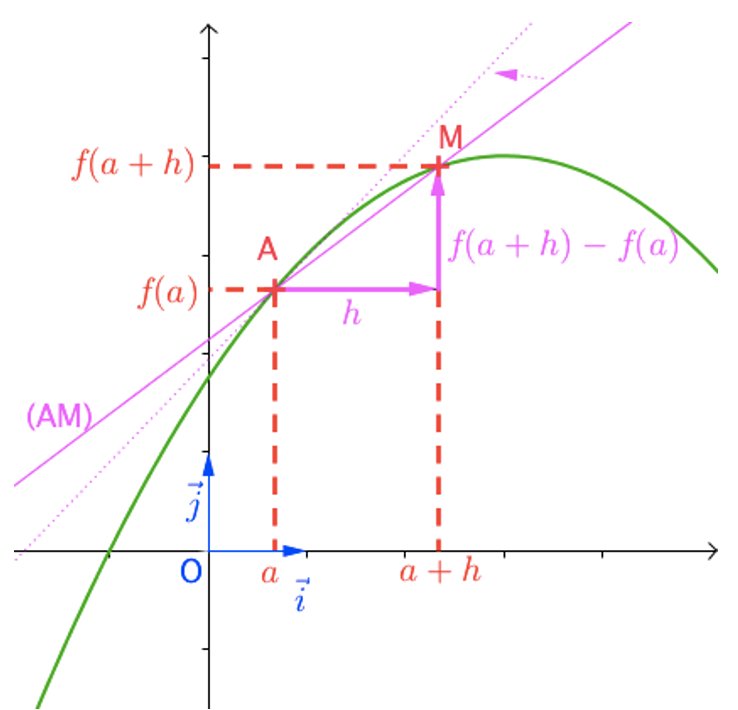
\includegraphics[scale=0.6]{01-05-Img03}

\end{multicols}

\begin{definition}
\phantom{$\dfrac{1}{3}$}\pointille[\textwidth-1cm]\\
\phantom{$\dfrac{1}{3}$}\pointille[\textwidth-1cm]\\
\phantom{$\dfrac{1}{3}$}\pointille[\textwidth-1cm]\\
\phantom{$\dfrac{1}{3}$}\pointille[\textwidth-1cm]
\end{definition}

\subsection{Démontrer qu'une fonction est dérivable}

\begin{bmethode}
    Soit la fonction trinôme $f$ définie sur $\mathbb{R}$ par $f(x)=x^{2}+2x-3$
    
    Démontrer que $f$ est dérivable en $x=2$.
    
    \phantom{$\dfrac{1}{3}$}\pointille[\textwidth-1cm]\\
\end{bmethode}

\section{Tangente à une courbe}

\subsection{Définition}

\begin{multicols}{2}
Soit une fonction $f$ définie sur un intervalle I et dérivable en un nombre réel $a$ appartenant à I.\\
$f^{\prime}(a)$ est le nombre dérivé de $f$ en $a$.\\
A est un point d'abscisse $a$ appartenant à la courbe représentative $C_{f}$ de $f$.

\begin{bdefi}
    \phantom{$\dfrac{1}{3}$}\pointille[\textwidth-1cm]\\
    \phantom{$\dfrac{1}{3}$}\pointille[\textwidth-1cm]\\
    \phantom{$\dfrac{1}{3}$}\pointille[\textwidth-1cm]\\
    \phantom{$\dfrac{1}{3}$}\pointille[\textwidth-1cm]
\end{bdefi}

\columnbreak

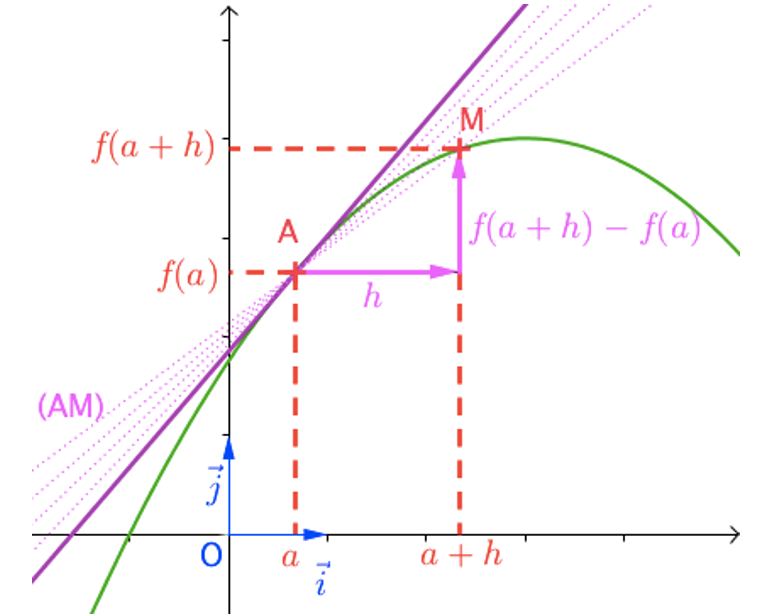
\includegraphics[scale=0.55]{01-05-Img04}
\end{multicols}

\subsection{Déterminer le coefficient directeur d'une tangente à une courbe}

\begin{bmethode}
    On considère la fonction trinôme $f$ définie sur $\mathbb{R}$ par $f(x)=x^{2}+2 x-3$ dont la dérivabilité en 2 a été étudiée plus haut.\\
    Déterminer la pente de la tangente à la courbe représentative de $f$ au point $\mathrm{A}$ de la courbe d'abscisse $2$.\\
    \phantom{$\dfrac{1}{3}$}\pointille[\textwidth-1cm]\\
    \phantom{$\dfrac{1}{3}$}\pointille[\textwidth-1cm]\\
    \phantom{$\dfrac{1}{3}$}\pointille[\textwidth-1cm]
    \begin{center}
        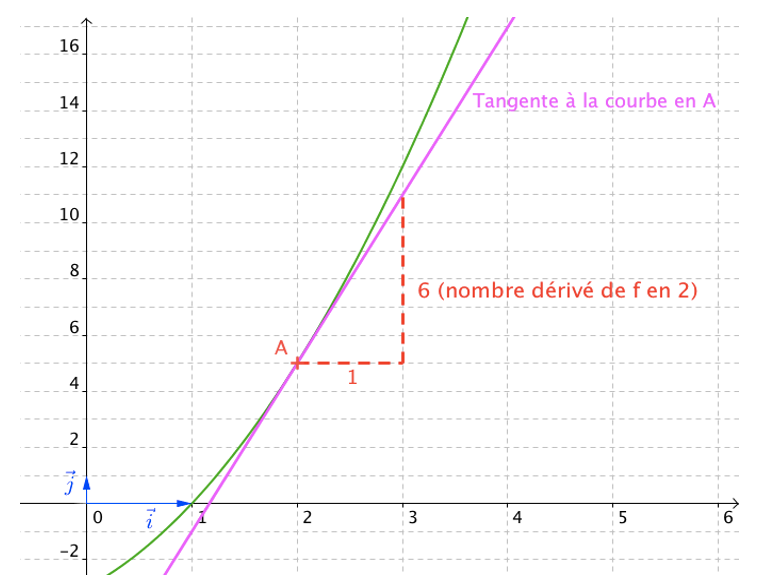
\includegraphics[scale=0.85]{01-05-Img05}
    \end{center}
\end{bmethode}

\subsection{Relation entre tangente et nombre dérivée}

\begin{bprop}
Une équation de la tangente à la courbe $C_{f}$ en A est :\\
\phantom{$\dfrac{1}{3}$}\pointille[\textwidth-1cm]\\
\end{bprop}

\begin{bdemo}
    \phantom{$\dfrac{1}{3}$}\pointille[\textwidth-1cm]\\
\end{bdemo}

\subsection{Déterminer une équation d'une tangente à une courbe}

\begin{bmethode}
    On considère la fonction trinôme $f$ définie sur $\mathbb{R}$ par $f(x)=x^{2}+2 x-3$.\\ Déterminer une équation de tangente à la courbe représentative de $f$ au point $\mathrm{A}$ de la courbe d'abscisse 2 .\\
   \phantom{$\dfrac{1}{3}$}\pointille[\textwidth-1cm]\\
   \phantom{$\dfrac{1}{3}$}\pointille[\textwidth-1cm]\\
   \phantom{$\dfrac{1}{3}$}\pointille[\textwidth-1cm]\\
   \phantom{$\dfrac{1}{3}$}\pointille[\textwidth-1cm]\\
   \phantom{$\dfrac{1}{3}$}\pointille[\textwidth-1cm]\\
\end{bmethode}

\section{Dérivées des fonctions usuelles}

\subsection{Exemple (démonstration au programme)}
\begin{bdemo}
    \phantom{$\dfrac{1}{3}$}\pointille[\textwidth-1cm]
\end{bdemo}

\begin{bdefi}
    \phantom{$\dfrac{1}{3}$}\pointille[\textwidth-1cm]\\
    \phantom{$\dfrac{1}{3}$}\pointille[\textwidth-1cm]\\
    \phantom{$\dfrac{1}{3}$}\pointille[\textwidth-1cm]\\
    \phantom{$\dfrac{1}{3}$}\pointille[\textwidth-1cm]\\
\end{bdefi}

\subsection{Formules de dérivation des fonctions usuelles}

% \begin{center}
%     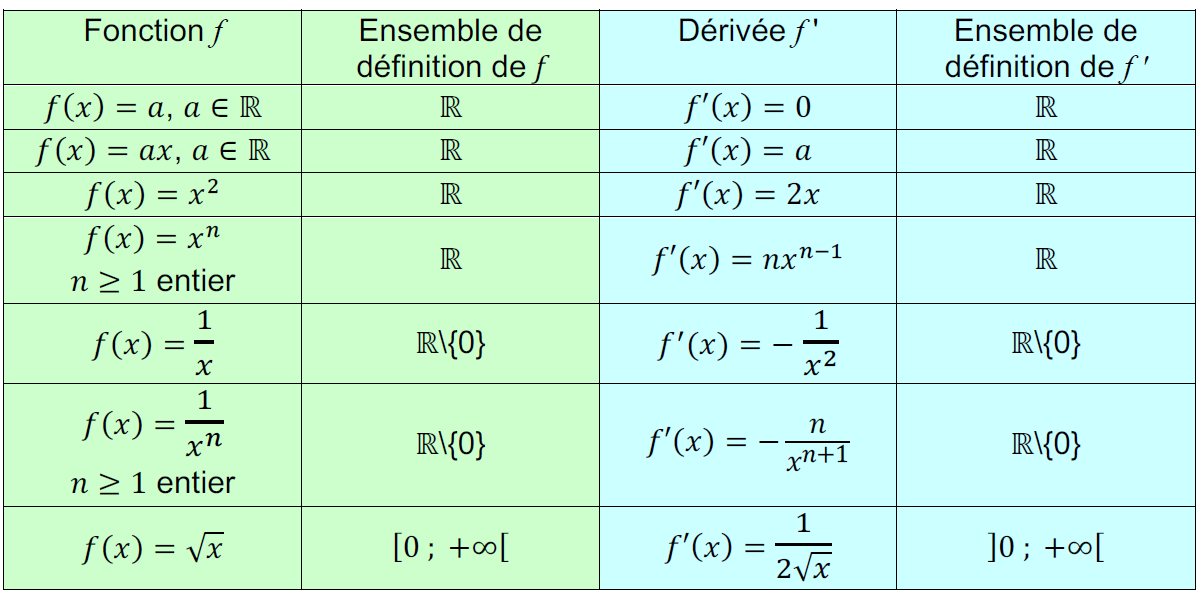
\includegraphics[scale=0.5]{01-06-01}
% \end{center}

\setlength{\arrayrulewidth}{1pt}
\renewcommand{\arraystretch}{1.9}
    \begin{tabular}{| >{\columncolor{green!25!white}}C{4cm} | >{\columncolor{green!25!white}}C{3cm} | >{\columncolor{cyan!25!white}}C{4cm} | >{\columncolor{cyan!25!white}}C{3cm} |}
\hline Fonction $f$ & Ensemble de\newline définition de $f$ & Dérivée $f^{\prime}$ & Ensemble de\newline définition de $f^{\prime}$ \\
\hline$f(x)=a$, $a \in \mathbb{R}$ & $\mathbb{R}$ & $f^{\prime}(x)=0$ & $\mathbb{R}$ \\
\hline$f(x)=a x$, $a \in \mathbb{R}$ & $\mathbb{R}$ & $f^{\prime}(x)=a$ & $\mathbb{R}$ \\
\hline$f(x)=x^{2}$ & $\mathbb{R}$ & $f^{\prime}(x)=2 x$ & $\mathbb{R}$ \\
\hline$f(x)=x^{n}$\newline $n \geqslant 1$ entier & $\mathbb{R}$ & $f^{\prime}(x)=n x^{n-1}$ & $\mathbb{R}$ \\
\hline$f(x)=\dfrac{1}{x}$ & $\mathbb{R} \backslash\{0\}$ & $f^{\prime}(x)=-\dfrac{1}{x^{2}}$ & $\mathbb{R} \backslash\{0\}$\rule[-7pt]{0pt}{30pt} \\
\hline$f(x)=\dfrac{1}{x^{n}}$\newline$n \geqslant 1$ entier & $\mathbb{R} \backslash\{0\}$ & $f^{\prime}(x)=-\dfrac{n}{x^{n+1}}$ & $\mathbb{R} \backslash\{0\}$ \\
\hline$f(x)=\sqrt{x}$ & {$[0 ;+\infty[$} & $f^{\prime}(x)=\dfrac{1}{2 \sqrt{x}}$ & ] $0 ;+\infty[$ \\
\hline
\end{tabular}

\begin{bexemples}
\begin{enumEx}
    \item Soit la fonction $f$ définie sur \R par $f(x)=x^4$ alors $f$ est dérivable sur \R et on a pour tout $x$ de \R, $f'(x)=4x^3$.
    \item Soit la fonction $f$ définie sur $\R \backslash \lbrace 0 \rbrace$ par $f(x)=\dfrac{1}{x^5}$ alors $f$ est dérivable sur $]-\infty ; 0[$ et sur $]0 ; +\infty[$ et on a pour tout $x$ de $\R \backslash \lbrace 0 \rbrace$, $f'(x)=-\dfrac{5}{x^6}$.
\end{enumEx}
\end{bexemples}

\subsection{Démonstration au programme pour la fonction inverse}

\begin{bdemo}
    \phantom{$\dfrac{1}{3}$}\pointille[\textwidth-1cm]
\end{bdemo}


\subsection{Démonstration au programme : Non dérivabilité de la fonction racine carrée en 0}

\begin{bdemo}
    \phantom{$\dfrac{1}{3}$}\pointille[\textwidth-1cm]
\end{bdemo}

\section{Opérations sur les fonctions dérivées}
\subsection{Somme, produit, inverse, quotient de dérivées}
\begin{bexemple}
    Soit la fonction $f$ définie sur \R par  $f(x)=x+x^2$.\\
    Pour $h\neq0$:\\ 
    \begin{align*}
    	\frac{f(a+h)-f(a)}{h}&=\frac{a+h+(a+h)^2-a-a^2}{h}\\
    	&=\frac{a+h+a^2+2ah+h^2-a-a^2}{h}\\
    	&=\frac{h+2ah+h^2}{h}=1+2a+h\\
    	&=1+2a+h\\
    \end{align*}
    \[ \text{Donc }:\lim\limits_{h \rightarrow 0} \frac{f(a+h)-f(a)}{h} = \lim\limits_{h \rightarrow 0} 1+2a+h=1+2a\]
    \\
    Alors $f$ est dérivable sur \R et on a pour tout $x$ de \R, $f'(x)=1+2x$.\\
    \\
    On pose pour tout $x$ de \R, $u(x)=x$ et $v(x)=x^2$. On a ainsi : $f(x)=u(x)+v(x)$.\\
    Pour tout $x$ de \R, $u'(x)=1$ et $v'(x)=2x$.\\
    On constate sur cet exemple que : $f'(x)=u'(x)+v'(x)$. Soit encore : $(u+v)'(x)=u'(x)+v'(x)$.
\end{bexemple}
\subsubsection{Formules d'opération sur les fonctions dérivées}
u et v sont deux fonctions dérivables sur un intervalle I.
%\begin{center}
%    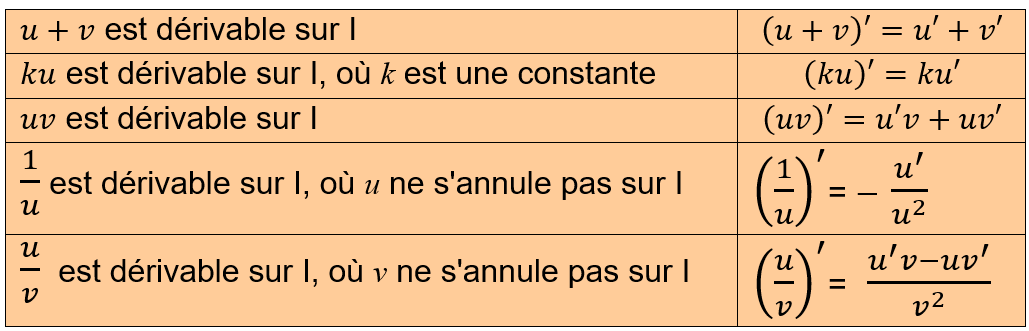
\includegraphics[scale=0.6]{01-06-03}
%\end{center}

\begin{center}
	%    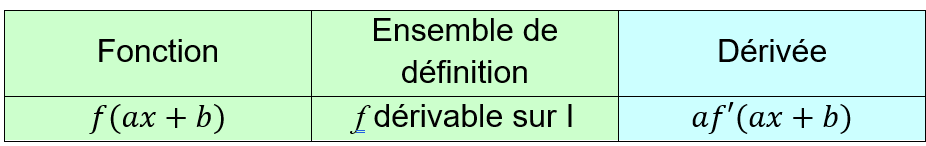
\includegraphics[scale=0.6]{01-06-04}
	\setlength{\arrayrulewidth}{1pt}
	\renewcommand{\arraystretch}{2.5}
	\begin{tabular}{| >{\columncolor{orange!25!white}}C{10cm} | >{\columncolor{orange!25!white}}C{5cm} | }
		\hline$u+v$ est dérivable sur I & $(u+v)'=u'+v'$ \\
		\hline$ku$ est dérivable sur I, où $k$ constante & $(ku)'=ku'$ \\
		\hline$uv$ est dérivable sur I & $(uv)'=u'v+uv'$ \\
		\hline$\dfrac{1}{u}$ est dérivable sur I, où $u$ ne s'annule pas sur I & $\left(\dfrac{1}{u}\right)'=-\dfrac{u'}{u^2}$ \\
		\hline$\dfrac{u}{v}$ est dérivable sur I, où $v$ ne s'annule pas sur I & $\left(\dfrac{u}{v}\right)'=\dfrac{u'v-uv'}{v^2}$ \\
		\hline
	\end{tabular}
\end{center}

\subsubsection{démonstration : Fonction dérivée d'un produit}
\begin{bdemo}
	\phantom{$\dfrac{1}{3}$}\pointille[\textwidth-1cm]
\end{bdemo}

\subsection{Calculer les dérivées de sommes, produits et quotients de fonctions}

\begin{bmethode}
Calculer les fonctions dérivées des fonctions suivantes :
\[\mBleu{1)}\ f_1(x)=5x^3\ \ \ \ \ \ \ \ \ \ \ \ \ \ \ \ \ \ \ \ \ \ \ \ \ \ \mBleu{2)} f_2(x)=3x^2+4\sqrt{x}\]
\[\mBleu{3)}\  f_3(x)=\dfrac{1}{2x^2+5x}\ \ \ \ \ \ \ \ \  \ \ \ \ \ \ \ \ \ \ \ \ \ \ \mBleu{4)}\ f_4 (x)=(3x^2+4x)(5x-1)\]

\phantom{$\dfrac{1}{3}$}\pointille[\textwidth-1cm]
\end{bmethode}


\subsection{Composée de dérivées}
\begin{center}
%    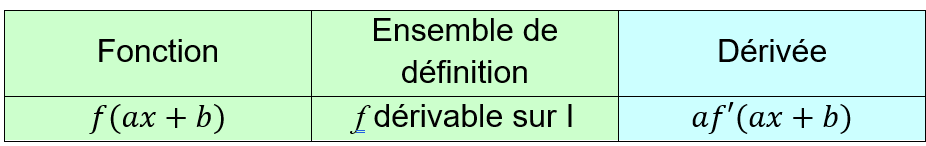
\includegraphics[scale=0.6]{01-06-04}
    \setlength{\arrayrulewidth}{1pt}
    \renewcommand{\arraystretch}{1.9}
    \begin{tabular}{| >{\columncolor{green!25!white}}C{4cm} | >{\columncolor{green!25!white}}C{4cm} | >{\columncolor{cyan!25!white}}C{4cm} | }
    	\hline Fonction & Ensemble de définition& Dérivée  \\
    	\hline$f(ax+b)$ & $f$ dérivable sur I & $af'(ax+b)$ \\
    	\hline
    \end{tabular}
\end{center}
\begin{bmethode}
    Calculer la dérivé des fonctions f et g suivantes : $f(x)=\sqrt{5x-4}$ et $g(x)=(4x-3)^5$\\		
    \phantom{$\dfrac{1}{3}$}\pointille[\textwidth-1cm]
\end{bmethode}

